% !TeX root = main.tex
% !TeX encoding = UTF-8
% !TeX spellcheck = en_GB
%=================================================================

Consider a probability space $(\Omega,\mathcal{F},P)$.

1. Let $\Omega$ be finite or countably infinite and let $\mathcal{F}$ be the powerset, set of all subsets of $\Omega$. In this situation \textit{random variables} are real-valued functions of $\Omega$.

2. In a more general probability space random variables are real-valued functions $X:\Omega \mapsto \mathbb{R}$ that satisfy:
$$\{\omega: X(\omega) \in (a,b)\} \in \mathcal{F}, \quad \forall a,b \in \mathbb{R}.$$

Random variables play a key role in probability and can be thought of as measurements of the outcome. Random variables, $X$, have a \textit{cumulative-distribution-function} associated with it: usually denoted by $F_X(x)$, defined as
$$ F_X(x):= P(\{\omega: X(\omega)\leq x\}), x \in \mathbb{R}.$$

There is a very important characterization theorem of cumulative distribution functions:

A function $G(x)$ is a cumulative distribution function \textit{if and only if} it satisfies the conditions:
\begin{enumerate}[$(i)$]
\item $G(x)$ is non-decreasing,
\item $\lim_{x \to -\infty} ~~ G(x) = 0, ~~~~~ \lim_{x \to +\infty} ~~ G(x) = 1$
\item $G(x)$ is right-continuous.
\end{enumerate}




In literature random variables are classified into \textit{discrete-random-variables} and \textit{continuous-random-variables}.

\begin{remark}
This classification is partly misleading since there are random variables that are neither discrete nor continuous. These are usually called mixed type.
\end{remark}

\textbf{Discrete-random-variables}: These are random variables that take values in a finite or a countable infinite subset of $\mathbb{R}$. If $\Omega$ is finite or countably infinite, then all random variables defined on this space will be discrete random variables.

Thus a discrete random variable $X$ take values in some subset $\{x_1, x_2, ...\}$ of $\mathbb{R}$. In this case, the cumulative distribution function is a non-decreasing piecewise-constant function that has discontinuities at $x_i$. Let $p_i = P(\{\omega:X(\omega)=x_i\})$, then we have
$$ F_X(x) = \sum_{i:x_i \leq x} p_i.$$
Observe that $F_X(x)$ has a "jump" of $p_i$ at value $x_i$.

Therefore, for discrete valued random variables, it is common to define a \textit{probability-mass-function (p.m.f.)}, $p_X(x)$ defined as:
$$ p_X(x_i) = p_i$$
and $p_X(x)=0 $ if $x \notin \{x_1,x_2,..\}.$


\textbf{Continuous-random-variables}: These are random variables, $X$, whose distribution function, $F_X$, is continuous in $\mathbb{R}$. For continuous random variables, it is common to define a \textit{probability-density-function}, $f_X$ (whose existence is beyond the scope of this class), satisfying
$$  F_X(x) = \int_{-\infty}^x f_X(y) dy.$$
Probability density functions are non-negative real-valued functions that integrate to one.

\section{Discrete Random Variables}
In this section we will study about some discrete random variables and their properties.

\textit{Notation}: For brevity we will say $P(X=x_i)$ instead of $P(\{\omega: X(\omega)=x_i\})$.

\begin{remark}
In reality, the above notation has its advantages. It is possible to talk of random variables, without really specifying the underlying probability space $(\Omega,\mathcal{F},P)$.
\end{remark}

\subsection{Some Common Examples}

\subsubsection{Bernoulli Random Variable} This is a random variable that takes two values $\{0,1\}$. As such it is used to distinguish whether an event $A$ or its complement $A^c$ has occurred.

We say $X \sim \textrm{Ber}(p)$, $p \in [0,1]$, if $p_X(1)=p$, and $p_X(0)=1-p.$

One should read $X \sim \textrm{Ber}(p)$ as $X$ is distributed according to a Bernoulli distribution with parameter $p$.

There are many examples where Bernoulli random variables arise naturally:
\begin{enumerate}
    \item Denote by 1 if the outcome of a coin toss is a head, and $0$ otherwise.
    \item Denote by $1$ if the roll of a dice results in an even number, $0$ otherwise.
\end{enumerate}

\subsubsection{Binomial Random Variable} This is a random variable that takes  values $\{0,1,2,...,n\}$.

We say $X \sim \textrm{Bin}(n,p)$, $p \in [0,1]$, if
$$ p_X(k)= \binom{n}{k}p^k(1-p)^{n-k},  0\leq k \leq n. $$
Observe that $\textrm{Bin}(1,p)$ has the same distribution as $\textrm{Ber}(p)$.

\subsubsection{Geometric Random Variable} This is a random variable that takes  values $\{1,2,...\}$.

We say $X \sim \textrm{Geo}(p)$, $p \in [0,1]$, if
$$ p_X(k)= (1-p) p^{k-1},  0\leq k, k \in \mathbb{N}. $$

\subsubsection{Poisson Random Variable} This is a random variable that also takes  values $\{0,1,2,...\}$.

We say $X \sim \textrm{Poi}(\lambda)$, $\lambda > 0$, if
$$ p_X(k)=  \frac{\lambda^{k}}{k!}e^{-\lambda},  0\leq k, k \in \mathbb{N}. $$

Consider binomial random variable $X_n \sim \textrm{Bin}(n, \frac{\lambda}{n})$ for some large $n$. Notice that the success probability $\frac{\lambda}{n}$ is small while the average number of success is a fixed number $\lambda$. By definition the p.m.f is
$$ p_X(k)= \binom{n}{k}\left( \frac{\lambda}{n}\right) ^k(1-\frac{\lambda}{n})^{n-k},$$
As $n\to \infty$, one can observe that the limit p.m.f is poisson p.m.f
\begin{align*}
\lim_{n\to \infty} \binom{n}{k}\left( \frac{\lambda}{n}\right) ^k(1-\frac{\lambda}{n})^{n-k} &= \lim_{n\to \infty}\frac{n(n-1) \ldots (n-k+1)}{k!}\frac{\lambda ^k}{n^k} (1-\frac{\lambda}{n})^{n-k}\\
&= \lim_{n\to \infty} \frac{\lambda^k}{k!} \left( 1\times (1-\frac{1}{n}) \times \ldots (1- \frac{k-1}{n})\right) (1-\frac{\lambda}{n})^{n} (1-\frac{\lambda}{n})^{-k}\\
&= \frac{\lambda^{k}}{k!}e^{-\lambda}
\end{align*}


\begin{remark}
A natural interpretation of the above four examples of discrete random variables is
\begin{itemize}
	\item Bernoulli random variable is to denote the outcome of a coin toss.
	\item Binomial random variable counts the number of heads in $n$ coin toss.
	\item Geometric random variable is the number of toss till the first tail occurs.
	\item Poisson random variable is the limit case of Binomial random variable for large number of toss but average success is fixed.  
\end{itemize}
\end{remark}

\subsection{Create discrete random variables}
\subsubsection{Truncated Geometric random variable}
Let $X \sim \textrm{Geo}(p)$. We can define $Y_n = \min\{X, n\}$. Then $Y$ is a discrete random variable taking values in $\{ 0, 1, \ldots, n\}$. The p.m.f of $Y_n$ is same as $X_n$ except
\begin{align*}
 p_{Y_n}(n) &= P(X\geq n)\\
 &= \sum_{k=n}^\infty (1-p) p^{k-1}\\
 &= p^{n-1}
\end{align*}

\subsubsection{Memoryless property of Geometric random variables}
Let $X \sim \textrm{Geo}(p)$ be the number of coin toss before first tail occurs. We can define $Y_n$ as the number of coin toss to get first tail given there are $n$ heads occurs already. Then the p.m.f of $Y_n$ is
\begin{align*}
	p_{Y_n}(k) &= P(X= n+k | X \geq n)\\
	&= \frac{P(X=n+k)}{P(X\geq n)}\\
	&= (1-p)p^{k-1}\\
	&= p_X(k)
\end{align*}
Observe that $P(X=n+k|X\geq n) = P(X=k) $. We call this memoryless property.


\section{Continuous Random Variables}
Random variables can take uncountably many, rather than discrete, values. We can define \textit{cumulative distribution function (c.d.f.)} of a random variable $X$,
$$F_X(x) = P(X \leq x)$$

It turns out c.d.f must satisfies the following three properties:
\begin{enumerate}
	\item $F_X(x)$ is non-decreasing function.
	\item As $x\to -\infty$, $F_X(x) \to 0$ and as $x \to \infty$, $F_X(x) \to 1$.
	\item $F_X(x)$ is right-continuous. i.e. $\lim_{x\to t^+} F_X(x) = F_X(t)$.
\end{enumerate}

We define \textit{continuous random variable} as random variables whose c.d.f $F_X(x)$ is continuouse \textit{every where}.

If $F_X(x)$ is differentiable, then the \textit{probability density function (p.d.f)} of $X$ is defined as
$$f_X(x) = \frac{dF_X(x)}{dx}$$

If $X$ has has p.d.f $f_X(x)$,
$$P(a\leq X \leq b) = \int_a^b f_X(t) dt$$

\subsubsection{Uniform random variable}
We say $X\sim \textrm{Unif} (a,b)$, for $a<b$, a uniform random variable if its c.d.f is 
$$F_X(x) = \begin{cases}
	0 & x < a\\
	\frac{x-a}{b-a} &  x \in [a,b] \\
	1 & x > b
\end{cases} $$
The distribution function is dipicted below \ref{fig:uniform}
\begin{figure}[h]
	\centering
	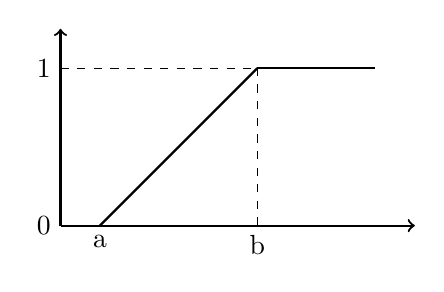
\begin{tikzpicture}
		\draw[thick,->] (0,0) -- (4.5,0);
		\draw[thick,->] (0,0) -- (0,2.5);
		\draw[thick] (0.5,0) -- (2.5,2);
		\node[below] at (0.5,0) {a};
		\draw[thick] (2.5,2) -- (4,2);
		\node[below] at (2.5,0) {b};
		\node[left] at (0,2) {1};
		\node[left] at (0,0) {0};
		\draw[dashed] (0,2) -- (2.5,2);
		\draw[dashed] (2.5,0) -- (2.5,2);
	\end{tikzpicture}
	\caption{Uniform distribution function}
	\label{fig:uniform}
\end{figure}

Its p.d.f is defined except at $x=a$ and $x=b$
$$f_X(x) = \begin{cases}
	\frac{1}{b-a} &  x \in [a,b] \\
	0 & \textrm{elsewhere}
\end{cases} $$

\subsubsection{Exponential random variables}
We say $X\sim \exp(\lambda)$ a exponential random variable if its c.d.f is
$$F_X(x) = 1 - \exp(-\lambda x), x\geq 0$$
and 0 elsewhere. It is dipicted below \ref{fig:exponential}

\begin{figure}[h]\centering
	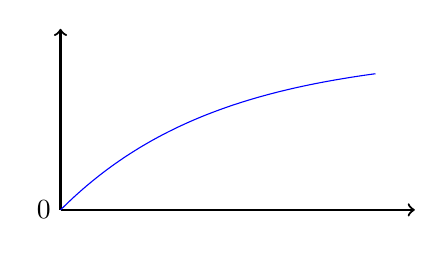
\begin{tikzpicture}
		\draw[thick,->] (0,0) -- (4.5,0);
		\draw[thick,->] (0,0) -- (0,2.3);
		\node[left] at (0,0) {0};
		\draw[scale = 2, domain=0:2, smooth, variable=\x, blue] plot ({\x}, {1-exp(-\x)});
	\end{tikzpicture}
	\label{fig:exponential}
	\caption{Exponential distribution function}
\end{figure}


\subsubsection{Guassian random variables}
We say $X\sim \mathcal{N}(\mu, \sigma^2)$ a Gaussian random variable if its p.d.f is
$$f_X(x) = \frac{1}{\sqrt{2\pi \sigma^2}} e^{-\frac{(x-\mu)^2}{2\sigma^2}}$$
The p.d.f is dipicted below \ref{fig:norm}
\begin{figure}[h]\centering
	\begin{tikzpicture}
		\draw[thick,->] (-3,0) -- (3,0);
		\draw[thick,->] (0,0) -- (0,2.7);
		\node[below] at (0,0) {0};
		\draw[scale=1.5, domain=-1.5:1.5, smooth, variable=\x, blue] plot ({\x}, {2*exp(-\x*\x*2)/sqrt(pi/2)});
	\end{tikzpicture}
	\label{fig:norm}
	\caption{p.d.f of $\mathcal{N}(0,1)$}
\end{figure}

\section{Random variable with discontinuous distribution function}
Consider a random variable $X$ be such that $X=0.5$ with probability 0.5 and $X\sim \textrm(Unif)(0,1)$ with probability 0.5. Then the c.d.f of $X$ is
$$F_X(x) =  \begin{cases}
	\frac{x}{2}, & \textrm{for $x\in [0, \frac{1}{2})$} \\
	\frac{1}{2} + \frac{x}{2}, & \textrm{for $x\in [\frac{1}{2}, 1]$}
	\end{cases}
$$


